\chapter{Implementation}

%The implementation should look at any issues you encountered as you tried to implement your design. During the work, you might have found that elements of your design were unnecessary or overly complex; perhaps third party libraries were available that simplified some of the functions that you intended to implement. If things were easier in some areas, then how did you adapt your project to take account of your findings?

%It is more likely that things were more complex than you first thought. In particular, were there any problems or difficulties that you found during implementation that you had to address? Did such problems simply delay you or were they more significant?

%You can conclude this section by reviewing the end of the implementation stage against the planned requirements.

\section{Image processing}
The image processing would prove to be an integral part of the application, enhancing the ability to learn handwriting more effectively and efficiently. The end script was implemented over a series of sprints.
\subsection{Optimising Tesseract}
After the design considerations to use OpenCV was chosen, specific algorithms would need to be implemented. After a discussion with Dr Hannah Dee, it was suggested that investigations into different binarisation scripts would be useful.

\subsubsection{OTSU}
[CITE CITE, Lab brooks page]

OTSU, created by Nobuyuki Otsu, is a binarisation technique which essentially converts an image to black and white. Otsu is a global thresholding algorithm, using the whole image as a comparsion. This is unlike local thresholding algorithms where comparisons are made pixel by pixel.CITE Automatic thresholding for defect detection].

Due to notes having non-uniform lighting by the intrusion of shadows on an image, this makes OTSU difficult to reliably binarise the image.

\begin{figure}[H]
  \centering
  \includdegraphics{images/OTSU}
  \label{fig:OTSU}
  \caption{The use of OTSU binarisation technique on an image with a little shadow across the image}
\end{figure}

Figure \ref{fig:OTSU} shows the binarisation technique on an image with the a slight shadow imposed on the image. Clearly it can be seen that it binarises the wrong sections of the image, this would be due to global thresholding.

The basic premise of OTSU is the image's grey-level values are segmented into a series of histograms. OTSU determines the optimial threshold value by ``maximising the discriminant measure''[CITE OTSU PAPTER][CITE OPENCV]. In other words, OTSU attempts to maximise the margin between the histograms. From the maximising of the histograms, pixels can be segmented into their background or foreground pixels. [CITE LAB BROOKS PAGE].

HP, who created Tesseract [CITE], describe OTSU as its underlying pre-processing algorithm when it tries to identify characters. From the iterative spike work with OTSU it is clear to see, just from Figure \ref{fig:OTSU}, how Tesseract would be unable to clearly identify characters from that image.

Overall, OTSU, although it is a very solid binarisation method, it suffers from imposed shadows over images. This would not be the best option to choose when choosing an appropriate binarisation technique.

\subsubsection{Adaptive Threshold}
From the enlighting analysis of OTSU it was realised that using an OTSU thresholding ontop of an OTSU threshold from the Tesseract engine would not be beneficial. Therefore, in the next iteration of the script, an adaptive threshold approach was chosen.

Adaptive threshold will calculate the threshold over a series of smaller segments of the image [CITE]. This reduces the impact of shadows over an image, and does not consider global illumination as the key.

Using the OpenCV library there was two options [CITE OPEN CV]:
\begin{enumerate}
  \item Gaussian adaptive threshold which is the weighted sum of the neighborhood
  \item Mean adaptive threshold, which is the mean of neighborhood.
\end{enumerate}

\begin{figure}[H]
  \centering
  \includegraphics{images/adaptivve_mean}
  \caption{Adaptive mean threshold algorithm on a note, showing binarisation but there is still noise in the image.}
  \label{fig:adaptive_mean}
\end{figure}

The mean neighboured takes a block size around the pixel, say 4, and will work out the mean pixel value from that block. The mean value selected will then be selected as the thresholding value, which will determine whether pixels are background or foreground. [CITE] Figure \ref{fig:adaptive_mean} shows a mean adaptive threshold. Due to smoothing issues there is still noise on the image.

The gaussian operation differs from the mean as it uses a gaussian value over the sub-image. Firstly each ``blocksize'' is a value which surround the pixel. A default gaussian weight is then calculated [ADD calculation] based on the blocksize. For every pixel in the block, multiply it by the gaussian, an average weight is then taken and used as a threshold. [CITE LEARN CV][CITE OPEN CV].


\begin{figure}[H]
  \centering
  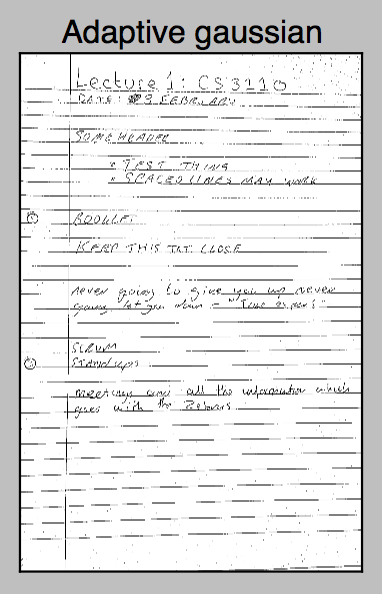
\includegraphics{images/adaptive_gaussian}
  \caption{Adaptive Gaussian used over the image, showing a lot smoother of an image}
  \label{fig:adaptive_gaussian}
\end{figure}

Figure \ref{fig:adaptive_gaussian} shows the adaptive gaussian shows an image which is working it's way to binarisation. It does not have a shadow overlaying the image and the text, lines and little noise have been extracted.

\begin{figure}[H]
  \centering
  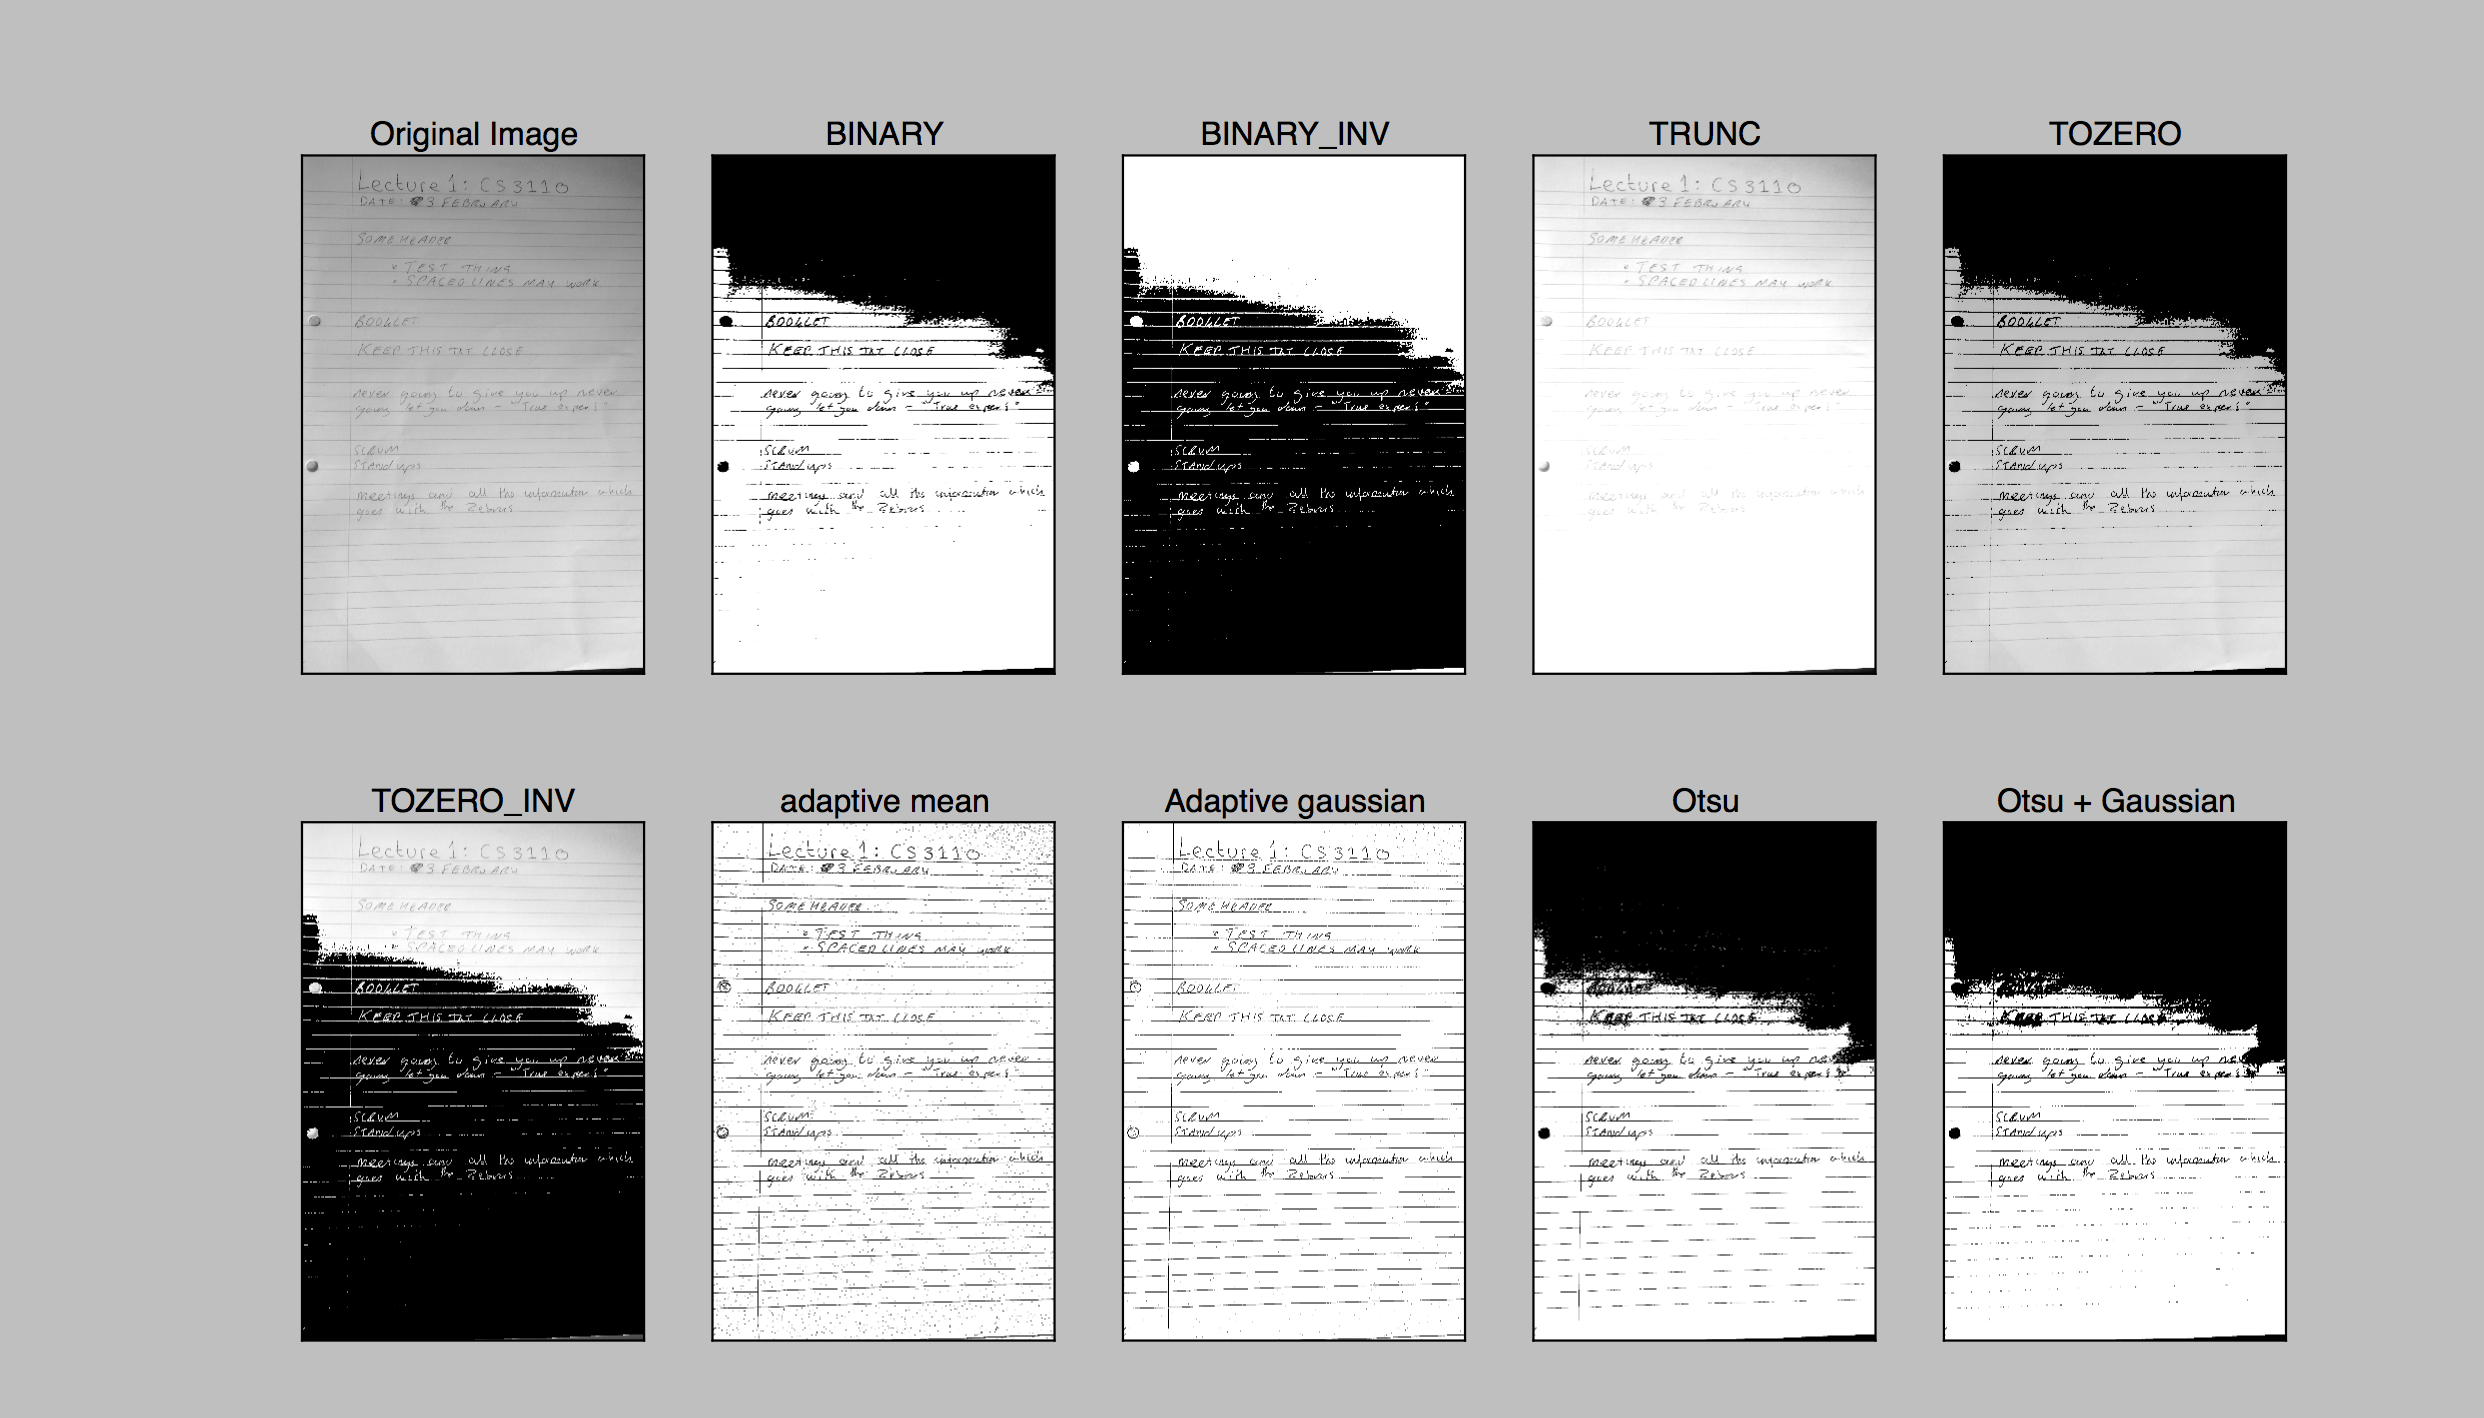
\includegraphics{images/thresholding_options}
  \caption{A variety of thresholding techniques used on the same note, showing adaptive threshold resulting in the best}
  \label{fig:thresholding_options}
\end{figure}

Figure \ref{fig:threshold_options} displays the other types of thresholding options iteratively tried. It was decided that the gaussian adaptive thesholding would be implemented and improved with different morphological operations.

\section{Lined paper}
Initially, standard lined paper was used; the noise that was produce was far too much to make Tesseract analyse characters correctly.

Due to Tesseract requiring text to be in horizontal lines [CITE HP PAPER] plain paper would often skew the text and make it harder for Tesseract to interpret the text.
\subsection{Filtering the blue lines}
As a result, custom blue lined paper Fig X, gives equal spacing between the lines as well as a horizontal structure. Blue was initially chosen as the pre-processing script would filter the blue lines and leave the black, binarised, text. The text would then appear as though it was written on normal paper and should not be included with the noise from the image.

This process went through a series of iterations to try and overcome issues identified through each iteration. The first process was to extract all the values on the page which fell between a predefined grey-black range. However, this had its obvious problems that it would extract some of the line where a dark blue would contain black-like elements of colour.

Morphological operations such as erroding [CITE] and dilation [CITE] was performed on the image, but to no avail - there was still noice in the image which causing Tesseract to interpret them incorrectly. This also had an unwanted side-effect: the binarised characters would then become so undistinguishable that they would not be able to be located correctly by the OCR tool. They became so pixelated that even from a human eye it was hard to identify their meaning.

\subsection{Only extracting the text}
The following optimisation would identify the lines, but only extract the text that was needed.
[CITE EXAMPLE ON OPEN CV]
A gaussian adaptive threshold operation was performed over a median blurred, grayscale version of the note; successfully binarising both the text and the lines. The horizontal lines on the page were extracted using OpenCV's structuring element, $MORPH\_RECT$ [CITE].

Further errosion and dilation was applied to remove the black lines and any noise residue from the extraction. A series of intermediate blank image masks were created to transfer the text from the image across to the mask. Although this carried all the text over, further line noise was also transferred across.

This suffered similar problems are the previous iteration, until connected components, via contours was discovered. Due to the morphological operations on the horizontal lines the connectivity between the pixels was very small. Thereby, choosing to use connected components would be able to extract the text from the image with little interference from the horizontal line noise. These connected components were then transferred to the new mask - only carrying the text from the image, not the lines.

Final morphological operations were included to improve the image quality. Overall the binarisation script works well.  It can take a photo of an image in a terrible light source Fig x, for example, and it would succesfully output the binarised image which would have distinguishable text, coinciding with little noise on the image. The noise on the image has little interference with the Tesseract OCR and it yields better results than greyscale images.
[CITE THE OPEN CV LYRIC EXAMPLE]
\section{Handwriting Training}
During the start of the handwriting training phase problems occurred such as it not reading the characters from a greyscale image correctly.
\subsection{Training process}
When using training data to be worked with Tesseract, it requires it to be in a specific file format. Such as: $<lang>.<font>.exp<number>.tiff$. When ran through a language, Tesseract outputs a box file which contains on each line: the character and the coordinates of this box. Trying to analyse this box was almost impossible. On the Tesseract wiki page [CITE] there's a link to jTessBoxEditor [CITE]. This tool was used to tag the boxes with their associated content.

Whilst using this editor the boxes could be expanded or shrunk to give the best possible fit to the characters. This was often utilised due to erroneous characters picked up by the editor.

There were a few issues when training the handwriting data, sometimes the data would not even be recongised.
% add some more stuff about training here.




\section{Web application}

\subsection{OAuth}
Working with the Google OAuth prooved to be quite tricky in some places. Using the Google client library to handle the OAuth2 interactions with the Google API's allowed for a reliable connection and exchanging of tokens.

During the interaction with the Google API's there was a time in which the API client failed and threw a random error. Confused as the service was working the prior day, an issue was made on their GitHub repository [CITE]. This issue miraculously dispearred after a clear of a cache from the API tool.

One issue to consider when dealing with OAuth is handling the refresh tokens. When a user authenticated, the credentials were stored in the user session. In the response from the Google OAuth is a refresh token - this has an expiration date. Prior to realising that the client had a check to see if the expiration token expired, the user would be presented with an error informing them they have an invalid token.

The new implementation redirects them to the logout url and asks them to re-authenticate.

\subsection{Reoccuring events}
Reocurring events were discovered as an issue in the pre-beta user testing. During the design phase when thinking about the calendar, it was forgotten that reocurring events and all-day events could exist.

All-day events do not have the dateTime key response from the Google Calendar API. As a result the code would fail when trying to access the dateTime from the event start date. This resulted in a redesign and re-think of the possible issues which could arise from Google Calendar.

Eventually, the dateTime key was checked and the all day events issue was solved.

However, the reocurring events problem was still existing. When querying for an event, if the event was reocurring then it would group the reocurring events by the first time in which the event was created. This resulted in an image, which was taken on the 12th March 2016 for example, to show events in February - if there was a reocurring event on the 12th March. However, it had an important reoccurence event ID key.

This resulted in a further query being created which would return all the instances that were reocurring. This had to pass in the $event['id']$ to the query to return all these instances; it was filtered down by querying for the start and end date.

When editing a reocurring event, Google calendar performs some unexpected behaviour: instead of silently modifying the event and returning the grouped event, again, it instead returns both the grouped event and the edited event. A succinct solution for this has not been found and has been a slight issue.

\subsection{Tesseract Confidence}
During a meeting with Dr Hannah Dee, it was suggested that some form of confidence score couldbe outputted to the user to show how well Tesseract identifies the text from the image.

The Tesseract command line does not output the confidence of the characters identified; only the C++ library can output the confidence. Due to time constraints, a wrapper for the C++ Tesseract API could not be implemented - so a third party library was chosen, tessocr[CITE].

Tessocr offered the implementation to access the confidence values for the associated words. The algorithm to execute the identification of the characters was quite simple.

Firstly we get all the text lines; Tesseract deals with the lines as a series of text lines. This is then enumerated over and for each line a corresponding list of confidence words is collected from tehe $map_all_words$ API.

Due to this returning a tuple which is an immutable object in Python, modifications on the list could not be made easily. This resulted in the view file checking the tuple content and calculating whether it is above the threshold; 75 for green, 70 for orange and below 65 for red.

\subsection{Displaying calendar events}

\subsection{Parsing Exif data}

\subsection{Editing calendar events}
When adding meta-data to a note, then the date which the user has entered is parsed into a query against the Google Calendar API which would return all the events for that day which they have entered. It would then check the module code entered against the summary field - this would ensure that the events would be found for that given module code.

This potentially displayed the problem of being able to add the note to the wrong event - if there was more than one event with the same module code that day. As a result a further check was conducted to evaluate the date start time and the date which they entered to ensure they matched.

If an event was matched then the event was added to the description field of a given saved note url. One issue which was discovered is that when adding a note it would just replace all the description with the note url and if they were editing it and it no longer existed then it would remove everything from the description. This is naturally bad, as it would mean that a user's description for an event would be overwritten.

This fixed with appending to the end of the description field, for the google calendar. Additionally, a replace was used instead of replacing with an empty string, this preserved the user's content in their description.



\section{Review against the requirements}
